\chapter{Introduction}

\begin{figure}[htbp]
\centering
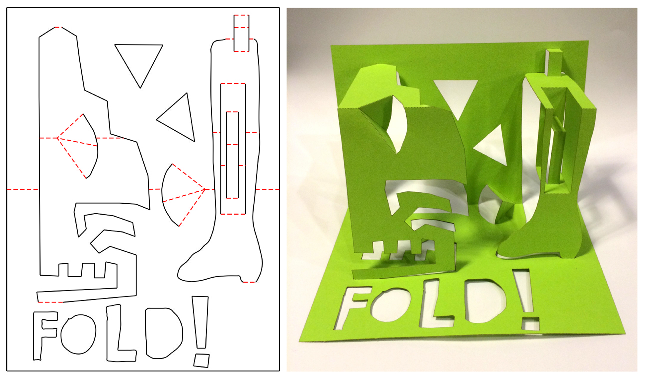
\includegraphics{figures/shared/01_Background/complexFoldlings.pdf}
\caption{A complex design created with our software.}
\end{figure}

\section{Background}\label{background}

\textbf{\textgreater{}\textgreater{}TODO: Complete w/Marissa} \emph{This
section is co-authored with Marissa Allen}

introduce kirigami, then popup cards, then maybe trees/graphs?

Kirigami is the art of papercraft originating from 17th century Japan
\citet{temko1978magic}. In contrast with origami, which only permits
folds, kirigami designs incorporate cuts. Thus, kirigami can represent a
wide range of 2D. Further In particular, Foldlings is concerned with
90-degree pop-up cards, which have the further constraint that
orthogonal relationships exist between planes. We do not use glue or
other attachment in building pop-up cards; all designs are cut from a
single piece of paper, in the tradition of kirigami
\citet{temko1978magic}.

\begin{figure}[htbp]
\centering
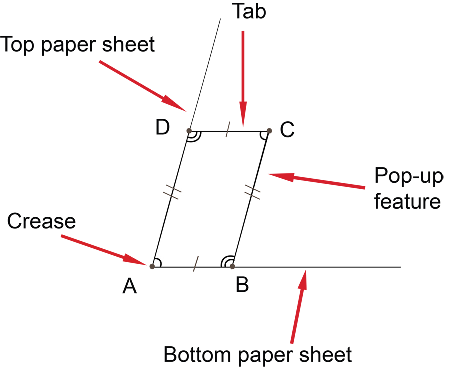
\includegraphics{figures/shared/01_Background/popup-diagram.pdf}
\caption{Cross-section of a popup card Figure modified from
https://en.wikipedia.org/wiki/File:Popup-diagram.svg.}
\end{figure}

The 90-degree popup card presents a tightly-constrained problem, with
opportunities for both interface design and algorithm innovations. We
present a system for designing popup cards, whose audience is
deliberately broad. We aim to make the pop=up card design process easier
and more fun.

Typically, users create popup cards through manual methods. For example,
a user might sketch out shape on a card in pencil, and then measure with
a rule to find locations to place folds. Or, they might \footnote{These
  are behaviors we observed by watching users create pop-up cards.}
